\documentclass[12pt]{beamer}
\usepackage[utf8]{inputenc}
\usepackage[spanish]{babel}
\usepackage{multirow}
\usepackage{color}
\usepackage{ragged2e}
\usepackage{movie15}


\mode<presentation>{\usetheme{CambridgeUS}}
\usecolortheme{dolphin}

\title[TASMC]{Traveler Assistant System For Mexico City TASMC}
\date{}

\begin{document}

\begin{frame}
	\begin{center}
	\begin{minipage}[t]{0.73\textwidth}	
		\begin{tabular}{ccc}
			\multirow{4}{*}{
\includegraphics[height=1.7cm]{imagenes/ipn.jpg}} &
			&
     	 	\multirow{4}{*}{
\includegraphics[height=1.5cm]{imagenes/escom.jpg}} \\
      		& Instituto Politécnico Nacional & \\
      		& Escuela Superior de Cómputo & \\
      		&&\\
		\end{tabular}
	\end{minipage}
	\end{center}
	
	\begin{center}
		\small No. de Registro: 2014-A021 \\
	\end{center}		
	
	\begin{center}
		\textcolor[RGB]{0,0,204}{\Large Traveler Assistant System For Mexico City TASMC}
	\end{center}		
		
	\begin{center}
	\begin{minipage}[t]{1\textwidth}	
		\begin{tabular}{ccc}
			Presentan & 
			\multirow{4}{*}{
\includegraphics[height=1.7cm]{imagenes/logo.png}} & Directores \\
			\scriptsize Barajas Uribe Sergio & & \scriptsize  M. en C. Macario Hernández Cruz\\
			\scriptsize Vivanco Carmona Erick Rafael & & \scriptsize M. en C. Axel Ernesto Moreno Cervantes
		\end{tabular}
	\end{minipage}
	\end{center}
\end{frame}

\section{Introducción}

\begin{frame}
	\frametitle{Introducción}
	\begin{block}{}
		\begin{itemize}
		\item Incremento de la transportación aérea.
		\item Creciente utilización de los dispositivos móviles.
		\item Adaptación a los nuevos usos de los dispositivos móviles.
		\item Dispositivo móvil + Internet = Enriquece la experiencia viajera.
	\end{itemize}
	\end{block}

\end{frame}

\subsection{¿Por qué TASMC?}
\begin{frame}
	\frametitle{¿Por qué TASMC?}
	\begin{columns} 
		\begin{column}{5cm} 
			\begin{block}{Necesidades} \small 
				\begin{itemize}
					\item Precio y horario de vuelos
					\item Buscar un hotel
					\item Hacer un itinerario de viaje
				\end{itemize} 
			\end{block} 
		\end{column}
		\begin{column}{5cm} 
			\begin{center}
				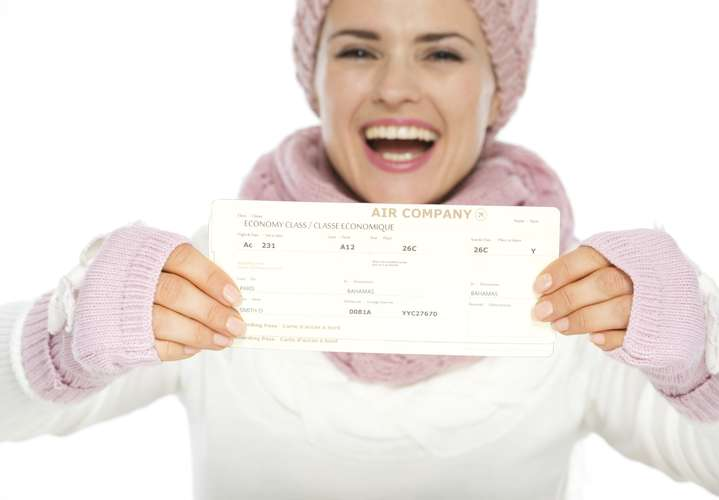
\includegraphics[height=2cm]{imagenes/nvuelo.jpg} \\
				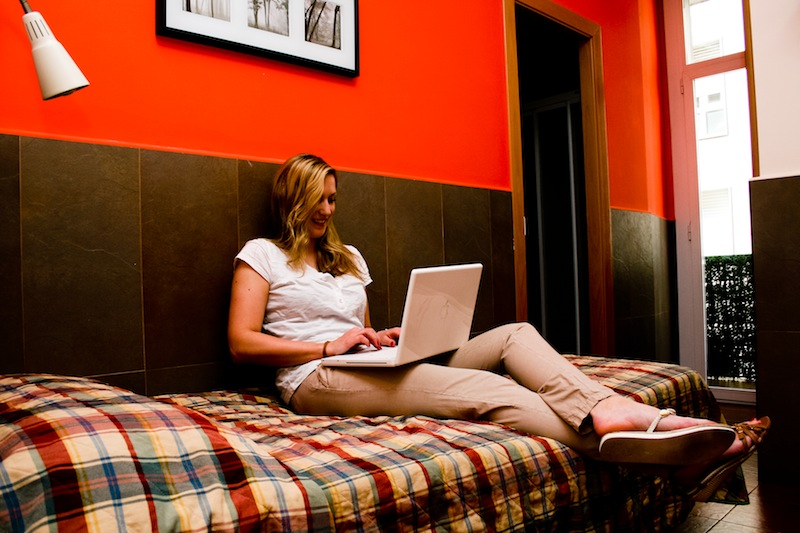
\includegraphics[height=2cm]{imagenes/nhotel.jpg} \\
				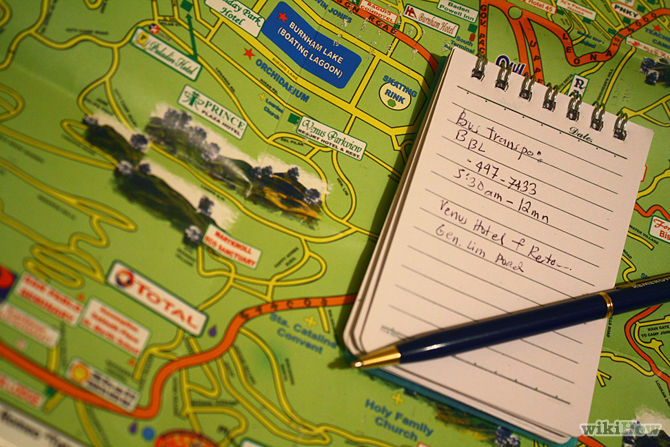
\includegraphics[height=2cm]{imagenes/nitinerario.jpg}
			\end{center} 
		\end{column} 
	\end{columns}
\end{frame}

\begin{frame}
	\frametitle{¿Por qué TASMC?}
	\begin{columns} 
		\begin{column}{5cm} 
			\begin{block}{Problemas} \small 
				\begin{itemize}
					\item Olvidar objetos 
					\item Llegar a destiempo al aeropuerto
					\item Perderse en el aeropuerto
				\end{itemize} 
			\end{block} 
		\end{column}
		\begin{column}{5cm} 
			\begin{center}
				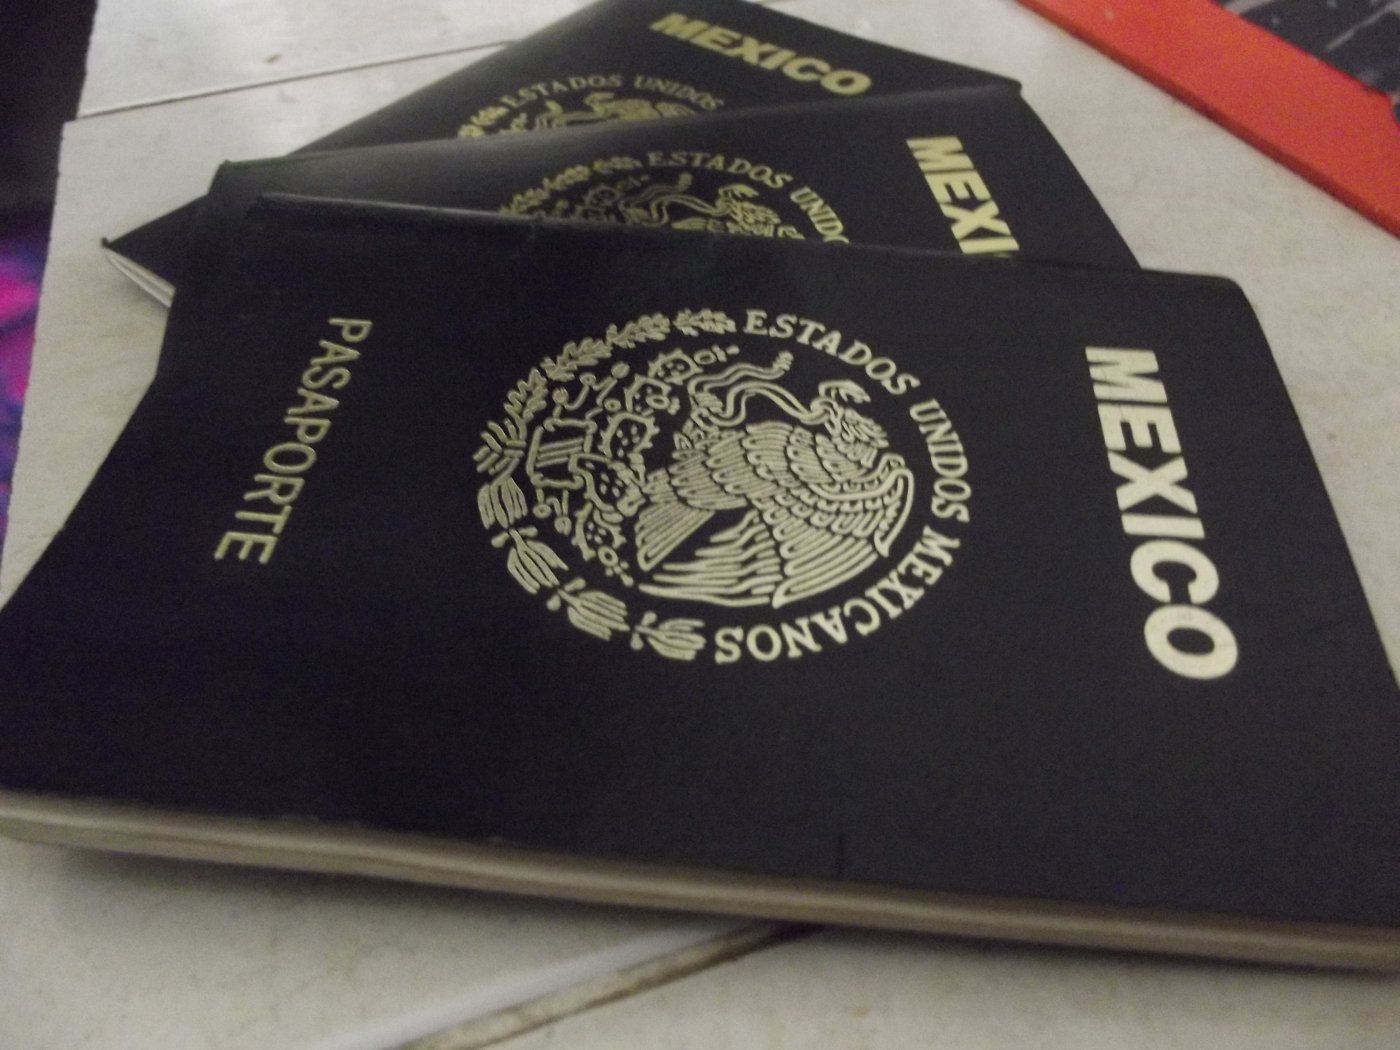
\includegraphics[height=2cm]{imagenes/pdocumento.jpg} \\
				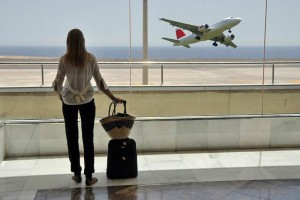
\includegraphics[height=2cm]{imagenes/pinpuntual.jpg} \\
				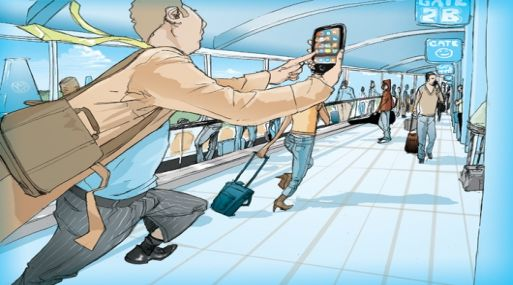
\includegraphics[height=2cm]{imagenes/pperderse.jpg}
			\end{center} 
		\end{column} 
	\end{columns}
\end{frame}

\subsection{¿Qué es TASMC?}
\begin{frame}[c]
	\frametitle{¿Qué es TASMC?}
	\begin{block}{}
		Sistema asistente para el viajero de la Ciudad de México
	\end{block}
	\begin{columns} 
		\begin{column}{5cm}
			\begin{block}{Características} \small 
				\begin{itemize}
					\item Configuración del viaje
					\item Vuelos disponibles
					\item Hoteles disponibles
					\item Lista de equipaje
					\item Itinerario de viaje
				\end{itemize} 
			\end{block} 
		\end{column}
		\begin{column}{4cm} 
			\begin{center}
				
\includegraphics[height=5cm]{imagenes/queEs.jpg}
			\end{center} 
		\end{column} 
	\end{columns}
\end{frame}

\begin{frame}[c]
	\frametitle{¿Qué es TASMC?}
	\begin{block}{}
		Sistema asistente para el viajero de la Ciudad de México
	\end{block}
	\begin{block}{}
	 	\textbf{AICM - } Aeropuerto Internacional de la Ciudad de México
	\end{block}
	\begin{columns} 
		\begin{column}{5cm}
			\begin{block}{Características} \small 
				\begin{itemize}
					\item Ruta al aeropuerto
					\item Ubicar dentro del AICM
					\item Información del vuelo
					\item Ruta del vuelo
				\end{itemize} 
			\end{block} 
		\end{column}
		\begin{column}{4cm} 
			\begin{center}
				
\includegraphics[height=5cm]{imagenes/queEs.jpg}
			\end{center} 
		\end{column} 
	\end{columns}
\end{frame}

\subsection{Objetivo de TASMC}

\begin{frame}
	\frametitle{Objetivo de TASMC}
	\begin{block}{}
		\justifying
		Diseñar un sistema integral de gestión para las actividades del viajero del AICM, al brindarle la información 						necesaria en su dispositivo móvil para hacer posible la organización integral del viaje e incentivar la demanda 					potencial de servicios de transportación aérea de viajes turísticos o de negocios en México.
	\end{block}
\end{frame}

\begin{frame}
	\frametitle{Arquitectura TASMC}
	\begin{center}
		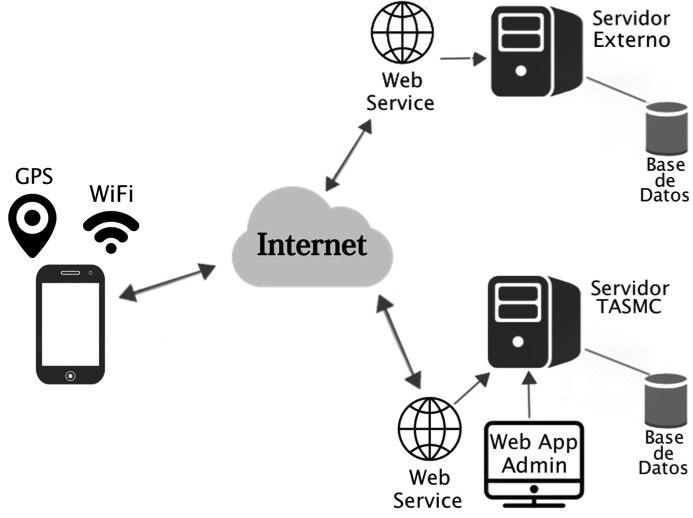
\includegraphics[height=6.5cm]{imagenes/arquitectura.png}	
	\end{center}
\end{frame}

\begin{frame}
	\frametitle{Interfaz Gráfica}
	\begin{block}{}
	\begin{center}
	
	 \includemovie[
  		poster,
  		text=(TASMC),
  		autorun]{1\linewidth}{0.5\linewidth}{tasmc.mp4}
  		\end{center}
   \end{block}
\end{frame}

\begin{frame}
	\frametitle{¿Qué necesitamos del AICM?}
	\begin{block}{} \small 
				\begin{itemize}
					\item Planos del AICM
					\item Acceso a servicios Web
					\item Información de los servicios
					\item Acceso a las salas de última espera
				\end{itemize} 
			\end{block} 
\end{frame}
	
\end{document}